\documentclass{article}

\usepackage{tikz}
\usetikzlibrary{arrows,automata}

\title{Some examples from {\em Theory of Computation}}
\author{Geoffrey Matthews}
\begin{document}
\maketitle

Put the following in your preamble:
\begin{verbatim}
\usepackage{tikz}
\usetikzlibrary{arrows,automata}
\end{verbatim}


Book's illustration:

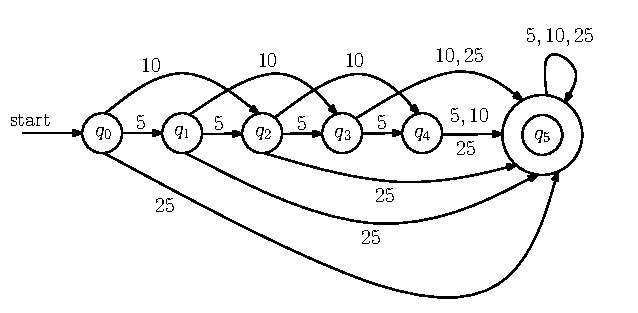
\includegraphics{p22.pdf}


Same thing done with tikz:

\newcommand{\nde}[2]{\node[state] (#1) [right of=#2] {$q_{#1}$};}
\begin{tikzpicture}[->,>=latex,auto,thick,node distance=2.5cm,every node/.style={scale=0.75}]
\node[initial,state] (0) {$q_0$};
\nde{1}{0}
\nde{2}{1}
\nde{3}{2}
\nde{4}{3}
\node[accepting,state] (5) [right of=4] {$q_5$};
\path (0) edge node {5} (1)
      (1) edge node {5} (2)
      (2) edge node {5} (3)
      (3) edge node {5} (4)
      (4) edge node {5,10,25} (5)
      (0) edge [bend left] node {10} (2)
      (1) edge [bend left] node {10} (3)
      (2) edge [bend left] node {10} (4)
      (3) edge [bend left] node {10,25} (5)
      (0) edge [bend right=40] node {25} (5)
      (1) edge [bend right=30] node {25} (5)
      (2) edge [bend right=20] node {25} (5)
      (5) edge [loop above] node {5,10,25} (5)
;
\end{tikzpicture}
\newpage

\begin{verbatim}  
  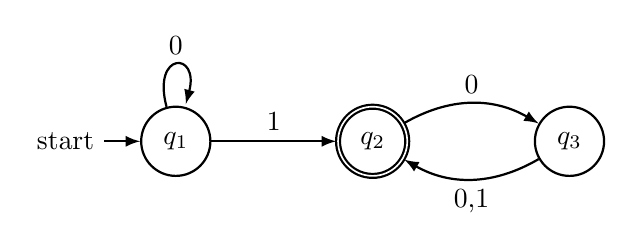
\begin{tikzpicture}[->,>=latex,thick,auto,node distance=2.5cm]
    \node[state,initial] (q1) {$q_1$};
    \node[state,accepting] (q2) [right of=q1] {$q_2$};
    \node[state] (q3) [right of=q2] {$q_3$};
    \path (q1) edge [loop above] node {0} (q1);
    \path (q1) edge node {1} (q2);
    \path (q2) edge [bend left] node {0} (q3);
    \path (q3) edge [bend left] node {0,1} (q2);
  \end{tikzpicture}
\end{verbatim}
  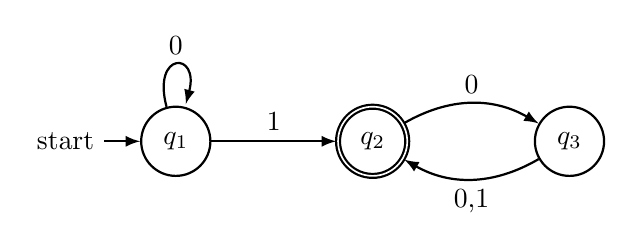
\begin{tikzpicture}[->,>=latex,thick,auto,node distance=2.5cm]
    \node[state,initial] (q1) {$q_1$};
    \node[state,accepting] (q2) [right of=q1] {$q_2$};
    \node[state] (q3) [right of=q2] {$q_3$};
    \path (q1) edge [loop above] node {0} (q1);
    \path (q1) edge node {1} (q2);
    \path (q2) edge [bend left] node {0} (q3);
    \path (q3) edge [bend left] node {0,1} (q2);
  \end{tikzpicture}
\begin{verbatim}  
  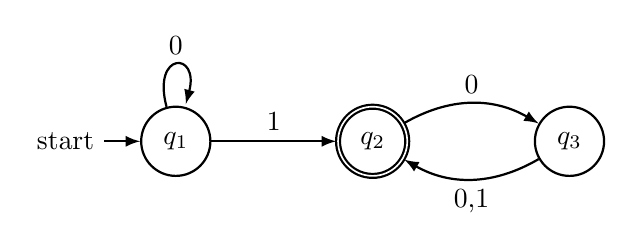
\begin{tikzpicture}[->,>=latex,thick,auto,node distance=2.5cm]
    \node[state,initial] (q1) {$q_1$};
    \node[state,accepting] (q2) [right of=q1] {$q_2$};
    \node[state] (q3) [right of=q2] {$q_3$};
    \path (q1) edge [loop above] node {0} (q1)
          (q1) edge node {1} (q2)
          (q2) edge [bend left] node {0} (q3)
          (q3) edge [bend left] node {0,1} (q2);
  \end{tikzpicture}
\end{verbatim}
  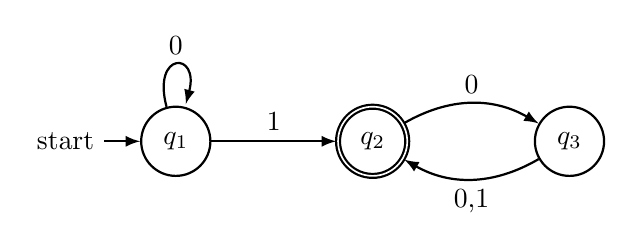
\begin{tikzpicture}[->,>=latex,thick,auto,node distance=2.5cm]
    \node[state,initial] (q1) {$q_1$};
    \node[state,accepting] (q2) [right of=q1] {$q_2$};
    \node[state] (q3) [right of=q2] {$q_3$};
    \path (q1) edge [loop above] node {0} (q1)
          (q1) edge node {1} (q2)
          (q2) edge [bend left] node {0} (q3)
          (q3) edge [bend left] node {0,1} (q2);
  \end{tikzpicture}

  \newpage
  
\begin{verbatim}  
  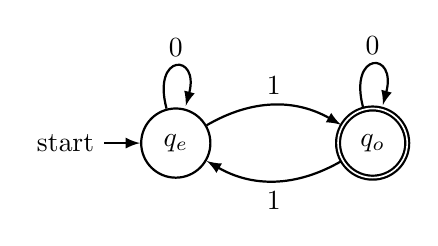
\begin{tikzpicture}[->,>=latex,thick,auto,node distance=2.5cm]
    \node[state,initial] (e) {$q_e$};
    \node[state,accepting] (o) [right of=e] {$q_o$};
    \path (e) edge [loop above] node {0} (e)
          (e) edge [bend left] node {1} (o)
          (o) edge [bend left] node {1} (e)
          (o) edge [loop above] node {0} (e);
  \end{tikzpicture}
\end{verbatim}
  
  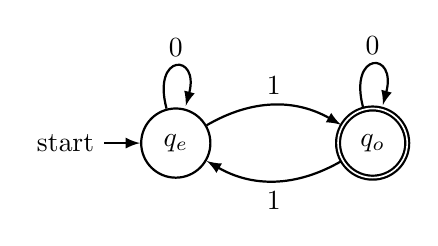
\begin{tikzpicture}[->,>=latex,thick,auto,node distance=2.5cm]
    \node[state,initial] (e) {$q_e$};
    \node[state,accepting] (o) [right of=e] {$q_o$};
    \path (e) edge [loop above] node {0} (e)
          (e) edge [bend left] node {1} (o)
          (o) edge [bend left] node {1} (e)
          (o) edge [loop above] node {0} (e);
  \end{tikzpicture}
  \begin{verbatim}
  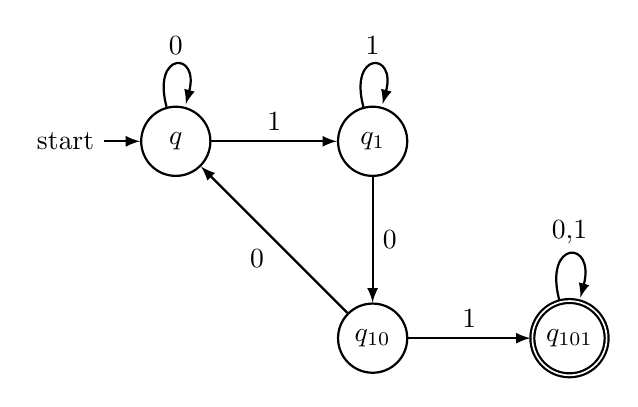
\begin{tikzpicture}[->,>=latex,thick,auto,node distance=2.5cm]
    \node[state,initial] (q) {$q$};
    \node[state] (1) [right of=q] {$q_1$};
    \node[state] (10) [below of=1] {$q_{10}$};
    \node[state,accepting] (101) [right of=10] {$q_{101}$};
    \path (q) edge [loop above] node {0} (q)
          (q) edge node {1} (1)
          (1) edge [loop above] node {1} (1)
          (1) edge node {0} (10)
          (10) edge node {0} (q)
          (10) edge node {1} (101)
          (101) edge [loop above] node {0,1} (101);
  \end{tikzpicture}
\end{verbatim}
  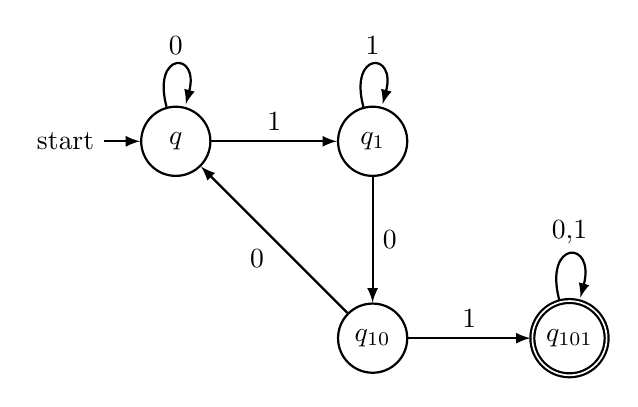
\begin{tikzpicture}[->,>=latex,thick,auto,node distance=2.5cm]
    \node[state,initial] (q) {$q$};
    \node[state] (1) [right of=q] {$q_1$};
    \node[state] (10) [below of=1] {$q_{10}$};
    \node[state,accepting] (101) [right of=10] {$q_{101}$};
    \path (q) edge [loop above] node {0} (q)
          (q) edge node {1} (1)
          (1) edge [loop above] node {1} (1)
          (1) edge node {0} (10)
          (10) edge node {0} (q)
          (10) edge node {1} (101)
          (101) edge [loop above] node {0,1} (101);
  \end{tikzpicture}





\end{document}
